\subsection{Error Artifacts}
\subsubsection{Confusion Matrix}
\begin{figure}[h]
    \centering
    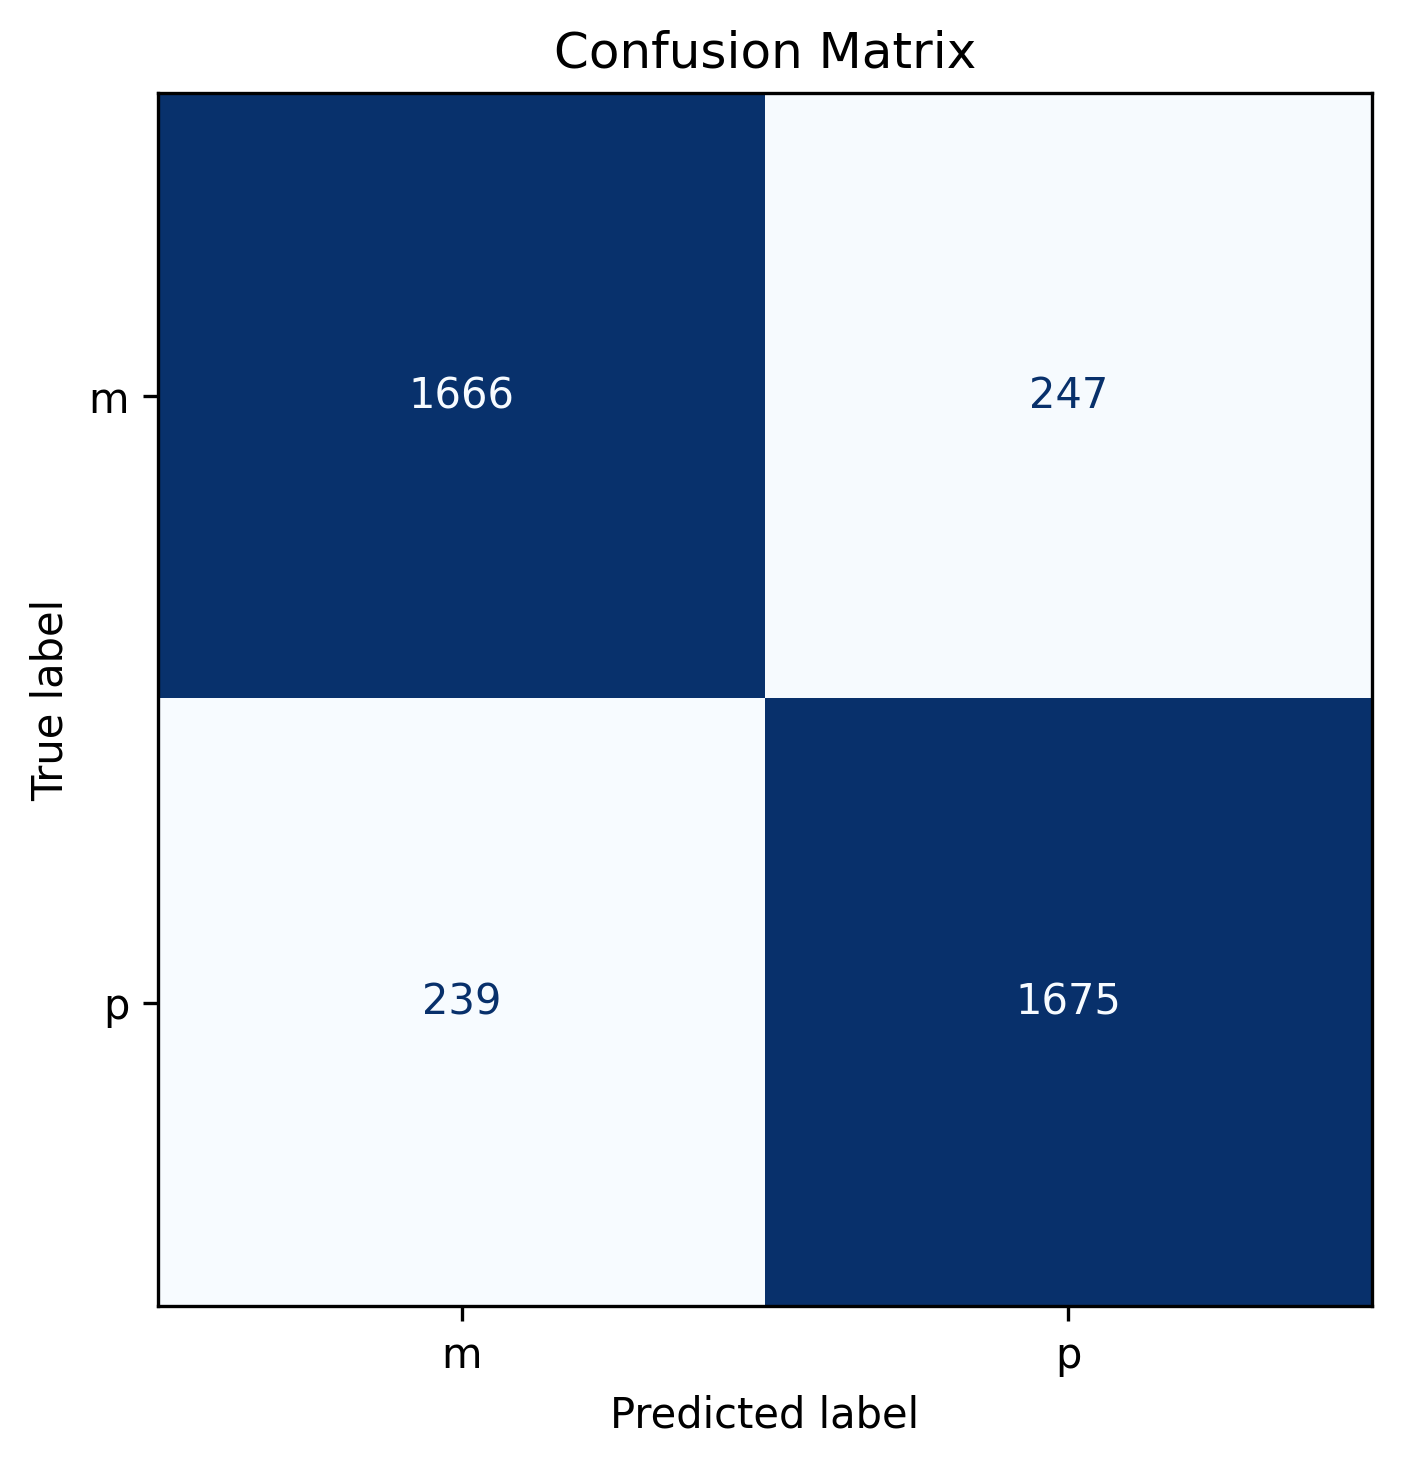
\includegraphics[width=0.4\textwidth]{assets/confusion_matrix_val.png}
    \caption{Confusion Matrix of LR+TF-IDF with Feature Engineering}
    \label{fig:example}
\end{figure}

Based on Figure 1, the confusion matrix shows that the model performs  well across both classes: Pop and Metal. Specifically, 1666 samples of Metal and 1675 samples of Pop were correctly classified. In contrast, only 247 samples of Metal lyrics and 239 samples of Pop were misclassified.

Most importantly, the almost equal error pattern conveys that the model does not exhibit a strong class bias for either genre. This is expected since a strongly balanced dataset distribution was used, as well as the model's intra-class performance (macro F1). The slightly higher correct predictions for Pop indicate marginally better separability for Pop lyrics, though the difference is minimal. Overall, the model appears strong at learning genre-specific lexical and stylistic signals while still encountering difficulty on lyrics with overlapping thematic vocabulary.

\subsubsection{Misclassified Samples}
\begin{table}[h]
\centering
\small
\begin{tabular}{rrrrrr}
\hline
\textbf{Lyric ID} & \textbf{True} & \textbf{Pred} & \textbf{Pred Conf.} & \textbf{Margin} & \textbf{Words} \\
\hline
87199 & m & p & 1.000 & 1.000 & 210 \\
69273 & m & p & 0.999 & 0.999 & 323 \\
5611  & p & m & 0.999 & 0.998 & 110 \\
92588 & m & p & 0.999 & 0.997 & 342 \\
89744 & p & m & 0.999 & 0.997 & 226 \\
82631 & m & p & 0.997 & 0.994 & 197 \\
5246  & m & p & 0.997 & 0.993 & 397 \\
11630 & p & m & 0.996 & 0.992 & 120 \\
7750  & m & p & 0.996 & 0.992 & 407 \\
87716 & m & p & 0.996 & 0.991 & 195 \\
\hline
\end{tabular}
\caption{Top Misclassified Lyric Samples}
\label{tab:misclassified_examples}
\end{table}

As shown in Table 2, the summary of misclassified samples was used to qualitatively analyze the most confident and incorrect model predictions. Specifically, using lyrics (based on lyric IDs) with the highest incorrect prediction confidence, we can identify samples where the model used the wrong features (i.e., lexical cues in the lyrics). Most importantly, after analyzing the textual features (lyrics) of each corresponding lyric ID, a common pattern is shown: the presence of emotional and intense vocabulary that overlaps between both Pop and Metal lyrics. This includes phrases related to pain, love, darkness or conflict. Considering these themes can appear in both genres, it is expected that the likelihood of model confusion with high prediction confidence increases. Moreover, since some songs consist of shorter or highly repetitive lyrics, the lower contextual information may cause additional ambiguity for the model during training and evaluation. As a result, the misclassified sample analysis may suggest that the residual errors of the model are caused by semantic overlap of themes (and related phrases) between the genres rather than issues with the model's parameters or training methodology. 

\subsection{Discussion}
The best performing model was the Logistic Regression model with further feature engineering, compared to the pretrained models tested. When analyzing the model's failures, a thematic challenge emerges regarding context and metaphor. The model was built using a robust feature pipeline that combined word and character n-gram TF-IDF vectors with custom numeric features (like type-token ratio, line counts, and punctuation usage). However, in instances such as song ID 114 and ID 1123, the model incorrectly guessed Pop for Metal songs because the lyrics centered on vulnerability and romance. Lines like "Light me a candle, I'm coming home / Then leave it on your side where I belong" (ID 114) and "Heartbreak and romance / It's better to be numb if you're cracking at the heart" (ID 1123) were misclassified because terms like "home," "heartbreak" and "romance" are statistically dominated by Pop music in the TF-IDF training data, overriding structural features and masking the heavier instrumentation that actually When the model incorrectly guessed Metal for a Pop song, as seen in ID 83472 and ID 60071, the lyrics relied heavily on aggressive metaphors. Lines like "Take away my prime from the mouth of the lion / Savage jaws are the price we pay" (ID 83472) and "Every spark has an ending like a burning fuse" (ID 60071) tricked the model because words like "lion," "savage," "jaws," and "burning" strongly trigger Metal classifications. The primary challenge here is that despite including structural features, the dominant TF-IDF vectors take words literally, failing to recognize when an aggressive word is just a metaphor for a pop breakup or when a soft word is sung over heavy, distorted guitars.

Despite these edge cases, the Logistic Regression pipeline is effective when songs lean into standard genre tropes. For example, a successful Pop classification for song ID 99344 ("head buster off top / grab the chopper and chop / at the top is my spot") demonstrates the model capturing rhythmic, upbeat language and modern slang typical of mainstream hip-hop/pop crossovers. On the other hand, a successful Metal classification for song ID 67457 ("Remnants strewn upon the ground / Drag the carcass withered and brown / Sockets crushed powder remaining") shows the model correctly identifying the overtly dark, morbid, and gothic vocabulary that serves as a staple of the metal genre. In these cases, the semantic meaning perfectly aligns with the literal definitions of the words, allowing the TF-IDF features to confidently and accurately predict the genre based purely on vocabulary frequency.

To improve the robustness of this model and eliminate the literal interpretation blindspots, future iterations should focus on moving beyond strictly frequency-based representations. Additionally, because lyrics only tell half the story, utilizing external APIs to include acoustic features such as energy, tempo, and instrumental features, alongside the existing custom numerical features would immediately resolve ambiguities between songs with similar lyrical themes but vastly different musical styles. 


Overall, the LR+TD-IDF model with feature engineering performs reasonably well with identifying and using correct lexical cues (within lyrics: textual features) for binary genre classification. 